\chapter{Background}\label{chapter:background}

\section{Regular Expressions}
Regular expressions (RegExp) are patterns used to search for character combinations in text using standardized concise syntax. A regular expression can specify both simple and complex character sequence patterns.  Table \ref{tab:regexsamp} shows examples of patterns and how they are represented as regular expressions.

{\renewcommand{\arraystretch}{1.6}% for the vertical padding
\begin{table}[H]
\centering
\begin{adjustbox}{width=1.1\textwidth,center=\textwidth}
\small
\begin{tabular}{|l|l|}
\hline
Pattern Description       & RegExp  \\
\hline
String starts with \textbf{hello} and ends in \textbf{world}. & \texttt{\textbf{\^{}hello.*world\$}} \\
\hline
Validate email address. & \texttt{\textbf{\^{}[A-Za-z0-9\_\%+-]+@[A-Za-z0-9.-]+.[A-Za-z]\{2,4\}\$}} \\
\hline
Any of the words \textbf{cat}, \textbf{dog} or \textbf{turtle}. & \texttt{\textbf{.*(cat|dog|turtle).*}}\\
\hline
\end{tabular}
\end{adjustbox}
\caption{Examples of Regular Expressions.}\label{tab:regexsamp}
\end{table}}

A regular expression is entered as a text string and is compiled into a tiny program designed specifically to identify that pattern by the regular expressions engine. This pattern can be used to find, search for, sub-string, or split text. Regular expressions are useful for a variety of tasks such as:
 \begin{itemize}
     \item \textit{Input validation}: e.g. to ensure that phone numbers are formatted correctly.
     \item \textit{Information search and extraction}: e.g. retrieving email addresses from documents. \item \textit{Advanced applications}: e.g. lexical analysis, network intrusion detection, and virus scanning.
 \end{itemize}

Regular expressions contain two types of characters:
\begin{enumerate}
    \item \textit{Literals} which are the actual characters to search, e.g. \texttt{\textbf{x}} will match the lower case character x.
    \item \textit{Meta-characters}: e.g. \texttt{\textbf{\^\$.*+}} are special characters that denote an operator that instructs the regex engine on how to match the other characters in the expression. Meta-characters allow regular expressions to be a powerful tool for text manipulation.
\end{enumerate}

We explore the meaning of each meta-character and the general syntax of Regular Expressions in detail in Section \ref{section:parser}. 


\section{Finite Automata}

Finite Automata (FA) or Finite State Machine (FSM) is an abstract machine for pattern recognition. It has a set of states and rules for transitioning from one state to the next depending on the input symbol used. It is essentially an abstract model of a digital computer. 

Finite Automata is defined formally as a 5-tuple, $(Q, Σ, T, q0, F)$ consisting of a finite set of states $Q$, a finite set of input symbols $\Sigma$, a transition function $T: Q \, x \, Σ → \, Q$, an initial state $q0 ∈ Q$, and accept states $F \subseteq Q$.

\begin{figure}[H]
\centering
\begin{tikzpicture}[->,>=stealth',shorten >=1pt,auto,node distance=3.5cm,scale = 1,transform shape]

  \node[state,initial] (p) {$q0$};
  \node[state] (s2) [right of=p] {$q1$};
  \node[state,accepting] (s3) [right of=s2] {$q2$};
  \node[state,accepting] (s4) [below of=s2] {$q3$};
  \node[state] (s5) [below of=s3] {$q4$};

  \path    (p) edge                          node {$a$} (s2);
  \path    (p) edge                          node {$b$} (s4);
  
  \path    (s2) edge                         node {$b$} (s3);
  \path    (s2) edge                         node {$a$} (s5);

  \path    (s3) edge                         node {$a, b$} (s5);

  \path    (s4) edge                         node {$a, b$} (s5);

  \path    (s5) edge                        [loop right] node {$a, b$} (s5);


\end{tikzpicture}
\caption{Example of a Finite Automata that recognizes the pattern \texttt{\textbf{ab}} or \texttt{\textbf{b}}.}
\label{fig:fsm}
\end{figure}

Finite Automata can represented be as a state transition diagram. Figure \ref{fig:fsm} shows a state transition diagram where $Q = \{q0, q1, q2, q3\}$, $\Sigma = \{a, b\}$, $F = \{q2, q3\}$. In the state transition diagram states are represented by circles. (The numbers inside the circles are labels to help with this conversation; they are not part of how the machine works.). A Finite Automata has two special states: the start state $q0$ and the matching states $F = \{q2, q3\}$. Start states are depicted with lone arrowheads pointing at them, and matching states are drawn as a double circle.

The machine works by reading the input string one character at a time transitioning from a state to another depending on the input character. When the input ends the machine checks if it ended in an accept state then it matches the string, Otherwise, If the machine ends in a non-matching state, it does not match the string. Following the transitions, the automata in Figure \ref{fig:fsm} recognizes either of these two patterns: \texttt{\textbf{ab}} and \texttt{\textbf{b}}.

The automata we have been discussing is called a deterministic finite automaton (DFA), because in any state, each possible input character transitions to at most one new state. There exists another type of Finite Automata called Nondeterministic Finite Automata (NFA) which is similar to DFA except:

\begin{itemize}
    \item Epsilon transitions ($\epsilon$) are allowed, i.e, it can transition from one state to another without reading an input symbol.
    \item It can transition to multiple state for a certain input.
\end{itemize}

\begin{figure}[H]
\centering
\begin{tikzpicture}[->,>=stealth',shorten >=1pt,auto,node distance=3.5cm,scale = 1,transform shape]

  \node[state,initial] (p) {$q0$};
  \node[state,accepting] (s5) [right of=p] {$q1$};


  \path    (p) edge                        [loop above] node {$a, b$} (p);
  \path    (p) edge                       node {$b$} (s5);


\end{tikzpicture}
\caption{Example of a Non-deterministic Finite Automata.}
\label{fig:nfafsm}
\end{figure}

Figure \ref{fig:nfafsm} shows an example of a Non-deterministic Finite Automata. At state $q0$ and reading $b$ the automata can either stay at $q0$ or transition to $q1$. In this case, when two or more transitions are applicable, the NFA "clones" itself into appropriately many copies, each one following a different transition. Therefore, simulating or following the NFA transitions can be exponential in the length of the pattern, i.e, $O(2^n)$.

However, the aforementioned features do not give NFA any additional power. When it comes to power, both are equivalent \cite{nfadfaeq}. In fact, every NFA can be converted to an equivalent DFA. In Subsection \ref{subsection:nfdtodfa}, we show an algorithm for conversion between NFA and DFA.

In the next section, we discuss how we can recognize a regular expression using finite automata.

\newpage
\section{RegExp Matching}

A RegExp engine is a computer program that takes an input a regular expression and input text to match.
It compiles the RegExp into a tiny program that is designed specifically to identify that pattern.
The program is then executed on the input text to look for matches.

Regular expressions engine are typically based on one of two algorithms for matching: Backtracking or DFA.

\subsection{Backtracking}

Backtracking is a general algorithm for solving certain computing problems. It builds candidates gradually to solutions and abandons a candidate (backtracks) when it thinks that the candidate cannot be completed to a valid solution.

Backtracking RegExp engine also called NFA matchers. They compile the regular expression into an equivalent non-deterministic finite automata. NFAs turn out to be exactly equivalent in power to regular expressions and every regex can be converted to an equivalent NFA and vice versa. After building the NFA, they directly simulate the NFA on the input text trying all possible transitions and backtracking when a transition does not lead to an accept state.

The problem with Backtracking is that its running time can be exponential, which simple implementations exhibit when matching against expressions contain both alternation and unbounded quantification and cause the algorithm to examine an exponential number of sub-cases.

Despite the exponential worst-case time guarantee, Backtracking offer significantly more flexibility and expressive capability. For example, any engine that supports the use of back-references must contain some form of backtracking.

\subsection{DFA Matching}

A deterministic finite automata based RegExp engine compiles the regular expression to an equivalent DFA. The DFA can be constructed explicitly and then run on the resulting input string one character at a time. DFA construction for a regular expression of length $n$ has an exponential worst-time guarantee $O(2n)$, but it has a linear match time, i.e, on a string of length $m$ it run in $O(m)$.


\section{Unicode}
The Unicode standard \cite{unicode} is a character encoding standard for multilingual written text that enables reliable and consistent worldwide text data interchange that aims to replace the numerous different ways of encoding characters with a single, universal, efficient and unambiguous standard.

The Unicode standard introduces three concepts to represent text:
\begin{enumerate}
    \item \textit{Code Point}: a unique number that maps to a specific character. It usually represents a single grapheme (visible symbols) but sometimes represents control characters, or formatting. The Unicode standard version 14.0 contains \textit{1,114,112} code points, most of which are available for encoding of characters.
    
    \item \textit{Code Unit}: a number that is used to encode and transmit Unicode text. A single code point is encoded by one or more code units. Each code unit is of the same size, which is determined by the encoding format.
    
    \item \textit{Unicode Transformation Format (UTF)}: an encoding format that can encode all of the possible character code points in Unicode. Version 14.0 of the Unicode standard defines three different UTF formats: (1) 32-bit UTF-32 (2) 16-bit UTF-16 and (3) 8-bit byte oriented UTF-8.
\end{enumerate}

\subsection{UTF-32}
UTF-32 is a \textit{fixed-length} encoding that uses 32-bit (4 bytes) to encode each code unit resulting in one code unit per code point. The main advantage of UTF-32 is constant time indexing of the text. On the other hand it is very space-inefficient since only twenty-one bits are needed to represent all Unicode characters so eleven bits will always be unused.

\subsection{UTF-16}
UTF-16 is a \textit{variable-length} extension to UCS-2 encoding which was a fixed-length 16-bit encoding. It uses one or two 16-bit code units to represent each code point. It is used as the text-encoding format by the Java programming language and JavaScript/ECMAScript. Despite that it never gained popularity on the web due to its incompatibility with ASCII encoding and is used by only 0.1\% of websites \cite{utf16usage}.

\subsection{UTF-8}
UTF-8 is \textit{variable-length} encoding that uses uses one to four 8-bit code units to represent each code point as shown in Table \ref{tab:utf8}. UTF-8 is the most popular encoding on the web \cite{utf8usage} due to its:
\begin{enumerate}
    \item \textit{Backward Compatibility}: Existing ASCII text is already valid UTF-8.
    \item \textit{Small Size}: A UTF-8 encoded file tends to be smaller than a UTF-16/UTF-32 encoded file since needs only at minimum single byte to represent a character and code points with lower numerical values, which are more frequent, are encoded using fewer bytes.
    \item \textit{Robustness}: If a code unit is corrupted, other characters will be processed correctly as it has been designed to recognize a code unit even if the previous code is not correct \cite{unicodeexplainedbook}.
\end{enumerate}

{\renewcommand{\arraystretch}{1.5}% for the vertical padding
\begin{table}[ht]
\centering
\begin{adjustbox}{width=1.1\textwidth,center=\textwidth}
\small
\begin{tabular}{|l|l|l|l|l|l|}
\hline
Code points        & Number of encoding bits & Code unit \#1 & Code unit \#2 & Code unit \#3 & Code unit \#4  \\
\hline
0x0000 - 0x007F & 7              & 0bbbbbbb &          &          &   \\
\hline
0x0080 - 0x07FF & 11 (5 + 6)     & 110bbbbb & 10bbbbbb &          &   \\
\hline
0x0800 - 0xFFFF & 16 (5 + 6 + 6) & 1110bbbb & 10bbbbbb & 10bbbbbb &   \\
\hline
0x10000 - 0xFFFFFF & 21 (5 + 6 + 6 + 6)      & 11110bbbb     & 10bbbbbb      & 10bbbbbb      & 10bbbbbb \\
\hline
\end{tabular}
\end{adjustbox}
\caption[UTF-8 Code Points Conversion]{UTF-8 Code point to Code unit Encoding.}\label{tab:utf8}
\end{table}}
The algorithm  for encoding UTF-8 \cite{utf8RFC} is as follows:
\begin{enumerate}
    \item Determine the number of code units required to represent the code unit from Table \ref{tab:utf8}. For example the Phi Symbol $\phi$ has code point \textbf{0x03C6} which falls in the second row range and is encoded using 2 code units.
    
    \item Prepare the high-order bits of the each code unit as per the table. Eg. for $\phi$ the first code unit starts with prefix \textbf{110} and the second code unit starts with \textbf{10}.
    
    \item Fill in the bits marked b from the bits of the code point number in binary by putting the lowest-order bits of
       the code point number in the lowest-order positions of the last
       code unit of the sequence.
\end{enumerate}

\begin{figure}[ht]
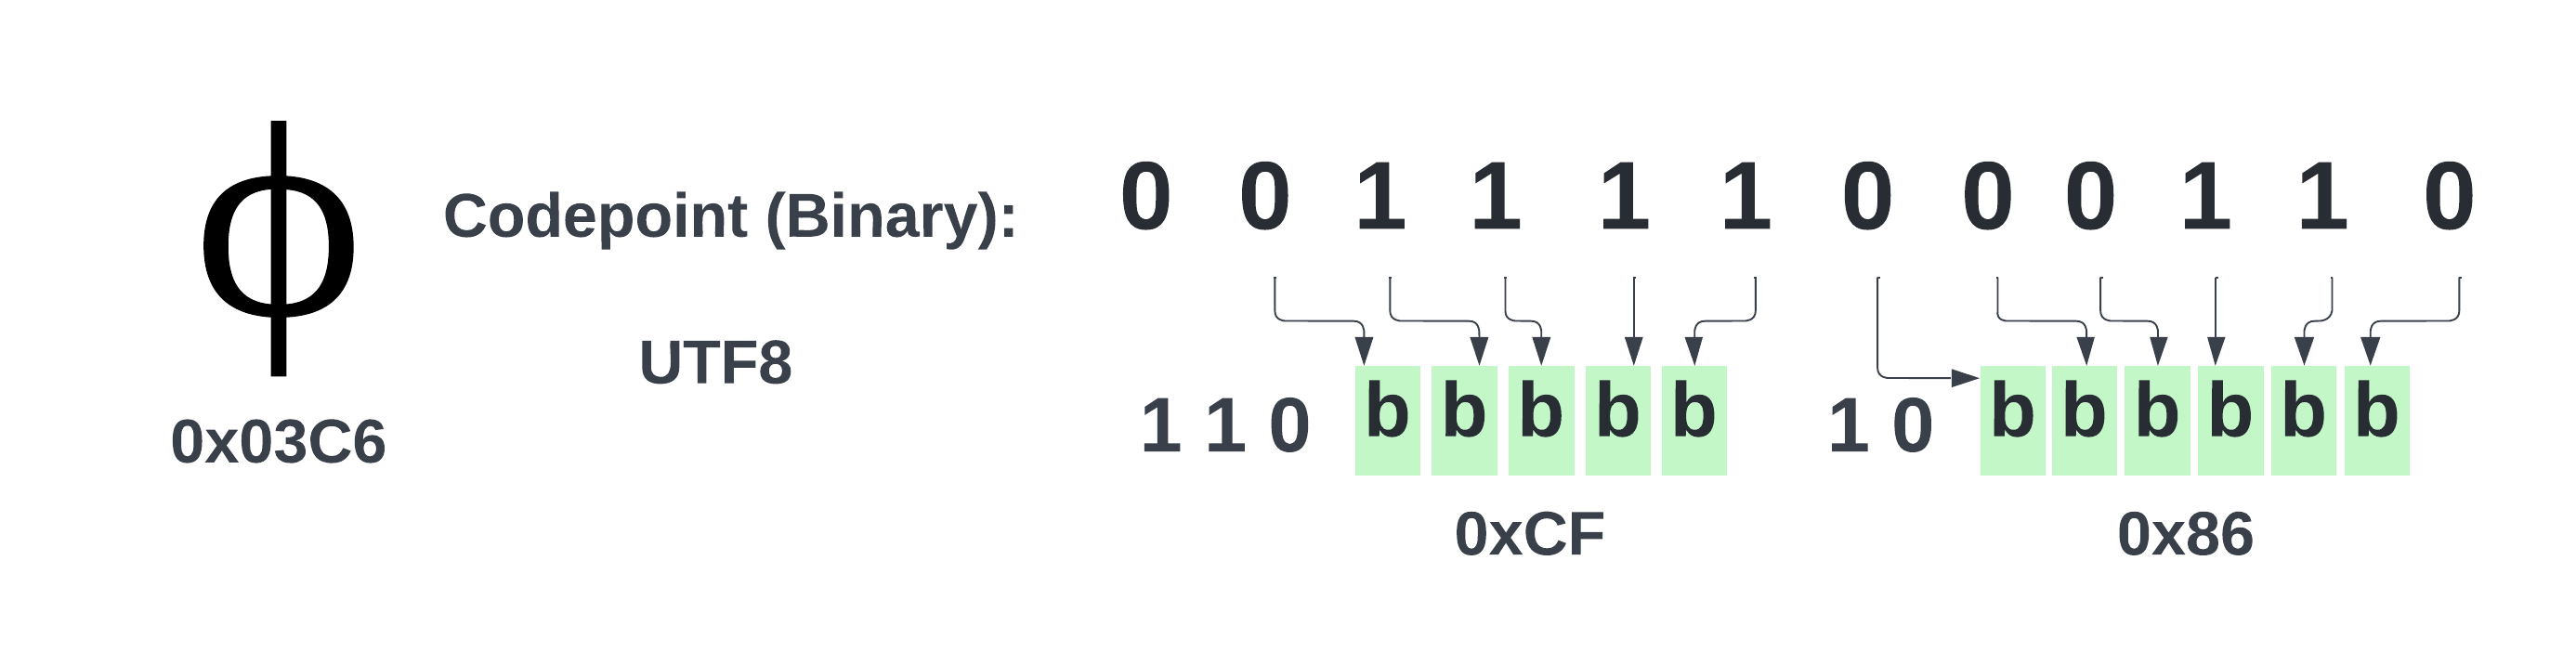
\includegraphics[trim=2cm 2cm 2cm 2cm,clip=true, width=\textwidth]{imgs/utf8-conv.png}
\caption[UTF8 Encoding]{UTF-8 Encoding for $\phi$ code point.}\label{fig:utf8-conv}
\end{figure}

For example applying the algorithm to encode the Phi Symbol $\phi$ which has a hex-decimal code point \textbf{0x03C6} which falls in the range of the second row in the table therefore it needs two code units. The high order code unit has prefix \textbf{110} which indicates that the code point is encoded with two bytes. The second code unit has prefix of \textbf{10}. The last step is to fill the remaining bits as show in Figure \ref{fig:utf8-conv}.
\section{LLVM}
LLVM (Low Level Virtual Machine) \cite{llvm} is a set of reusable modular compiler tools that originated as a University of Illinois research project in 2003 with the purpose of developing a modern, SSA (Static Single Assignment) based compilation framework capable of enabling both static and dynamic compilation of arbitrary programming languages.

The LLVM assembly language is based on a powerful language-independent intermediate code representation (IR) that is light-weight, type safe with strictly defined semantics, flexible and low-level enough to be capable of representing high-level languages cleanly. Based on that it can be used to create a compiler front-end or a back-end for any ISA (Instruction Set Architecture). LLVM also includes compiler front-ends for the C and C++ programming languages that competes with GCC in terms of compilation speed and performance \cite{llvmgcc}.

\begin{figure}[ht]
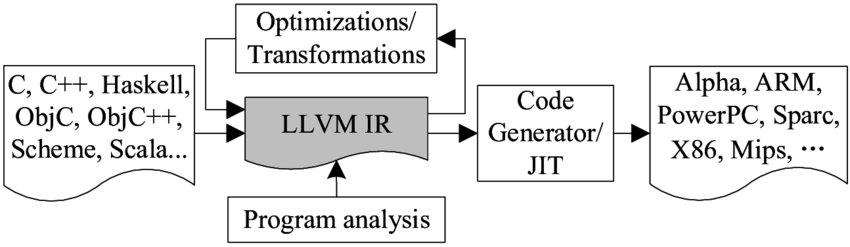
\includegraphics[width=\textwidth]{imgs/llvm-arch.png}
\caption[LLVM Compiler Infrastructure]{LLVM Compiler Infrastructure \cite{llvminfra}}\label{fig:llvminfra}
\end{figure}

The process of translating from high-level source code to executable machine-code by an LLVM-based compiler front-end summarized in Figure \ref{fig:llvminfra} is as follows:
\begin{enumerate}
    \item High-level source code is translated to LLVM IR. LLVM provides tools and APIs for the translation.
    \item The LLVM IR is further transformed and optimized using the LLVM aggressive optimizer that performs scalar, interprocedural, profile-driven, and some simple loop optimizations.
    \item LLVM compiler compiles the IR to machine code. The LLVM IR Compiler supports a variety of target architectures (e.g x86, ARM, ...) and provides both static and dynamic JIT-compilation.
\end{enumerate}

\subsection{Static Single Assignment (SSA)}
A program is said to be in Static Single Assignment (SSA) \cite{ssa} form if and only if all variables are assigned and every variable be defined before it is used. SSA simplifies and enhances the results of a multitude of compiler optimizations and is standard for intermediate representations (IR) in compilers of imperative programming languages. Therefore, A valid LLVM IR must be in SSA form.

\noindent The conversion of ordinary program code into SSA form follows two rules:
\begin{enumerate}
    \item The compiler replaces any assignment to an already-assigned variable with a brand new “version” of that variable e.g variable \texttt{\textbf{$x$}} becomes \texttt{\textbf{$x_1$}}
    \item The compiler uses Phi function ($\phi$) to introduce a new variable when it needs to choose a variable based on control flow.
\end{enumerate}

Listing \ref{lst:cfgcode} shows an example code snippet of a program that is not in SSA form with respect to the variables $a, b, c$.

\begin{listing}[htbp]
\begin{minted}[breaklines=true,frame=lines,linenos]{cpp}
a = 3;
a = a - 1;
if (a > 0) {
 b = a * 2;
 c = b;
} else {
 b = a - 1;
}
c = a - b;
d = a + b;
\end{minted}
\caption{Code Snippet for a program \textit{not} in SSA form.}
\label{lst:cfgcode}
\end{listing}

The code in Listing \ref{lst:cfgcode} can be represented as a Control Flow Graph (CFG) as shown in Figure \ref{fig:cfg1}. A Control Flow Graph (CFG) is a graph representation of all paths that can be traversed by a program during its execution. The CFG consists of four nodes representing the entry node, two nodes one for each path for the control-flow condition $a > 0$ and the exit block.

\tikzset{bignode/.style={rectangle, draw, minimum size=4em,align=center}}

\begin{figure}[H]
\centering
\usetikzlibrary{shapes,calc}
\begin{tikzpicture}[->,>=stealth',shorten >=1pt,auto,node distance=3cm,scale = 1,transform shape]
  \node[bignode] (b0) {$a = 3;$\\$a = a - 1;$\\$(a > 0)$};
  \node[bignode] (b1) [below left of=b0]{$b = a * 2;$\\$c = b;$};
  \node[bignode] (b2) [below right of=b0]{$b = a - 1;$};
  \node[bignode] (b3) [below right of=b1] {$c = a - b;$\\$d = a + b;$};

  \path[->] (b0) edge (b1);
  \path[->] (b0) edge (b2);
  \path[->] (b1) edge (b3);
  \path[->] (b2) edge (b3);

\end{tikzpicture}\caption{CFG for source code in Listing \ref{lst:cfgcode}.}
\label{fig:cfg1}
\end{figure}

Applying the first rule to the code and giving distinguishing subscripts to all the variables results in the introduction of new variables ${a_2, b_2, c_2}$. We also renamed the old variables to ${a_1, b_1, c_1}$ for clarity. The resulting CFG is shown in Listing \ref{fig:cfg2}.

\begin{figure}[H]
\centering
\usetikzlibrary{shapes,calc}
\begin{tikzpicture}[->,>=stealth',shorten >=1pt,auto,node distance=3cm,scale = 1,transform shape]
  \node[bignode] (b0) {$a_1 = 3;$\\$a_2 = a_1 - 1;$\\$(a_2 > 0)?$};
  \node[bignode] (b1) [below left of=b0]{$b_1 = a_2 * 2;$\\$c_1 = b_1;$};
  \node[bignode] (b2) [below right of=b0]{$b_2 = a_2 - 1;$};
  \node[bignode] (b3) [below right of=b1] {$c_2 = a_2 - b_?;$\\$d_1 = a_2 + b_?;$};

  \path[->] (b0) edge (b1);
  \path[->] (b0) edge (b2);
  \path[->] (b1) edge (b3);
  \path[->] (b2) edge (b3);

\end{tikzpicture}\caption{CFG after applying the first SSA transformation rule.}
\label{fig:cfg2}
\end{figure}

We see only one problem in the CFG shown in Figure \ref{fig:cfg2} depending on the path the control flow went, both usage of $b$ in the bottom block might be referring to either $b_1$ or $b_2$. To resolve this we apply the second rule and use the Phi function to choose the right value, depending on the control flow.

Figure \ref{fig:cfg3} shows the CFG after applying the rule. We insert a special function call to the Phi function that will generate a new definition of b named $b_3$ that chooses either $b_1$ or $b_2$, based on the control flow in the past. We can then use $b_3$ in the last two statements and we are sure the correct value of $b$ will be used.
Calculating the value of the Phi function for an arbitrary control-flow graph is a difficult task but has an efficient algorithm \cite{domalgo}.

\begin{figure}[htbp]
\centering
\usetikzlibrary{shapes,calc}
\begin{tikzpicture}[->,>=stealth',shorten >=1pt,auto,node distance=3cm,scale = 1,transform shape]
  \node[bignode] (b0) {$a_1 = 3;$\\$a_2 = a_1 - 1;$\\$(a_2 > 0)?$};
  \node[bignode] (b1) [below left of=b0]{$b_1 = a_2 * 2;$\\$c_1 = b_1;$};
  \node[bignode] (b2) [below right of=b0]{$b_2 = a_2 - 1;$};
  \node[bignode] (b3) [below right of=b1] {$b_3 = \phi(b_1, b_2);$\\$c_2 = a_2 - b_3;$\\$d_1 = a_2 + b_3;$};

  \path[->] (b0) edge (b1);
  \path[->] (b0) edge (b2);
  \path[->] (b1) edge (b3);
  \path[->] (b2) edge (b3);

\end{tikzpicture}\caption{CFG after applying the second SSA transformation rule.}
\label{fig:cfg3}
\end{figure}


\subsection{Jit Compilation}
Just-in-time (JIT) is dynamic compilation method for programs that involves compilation during a program's execution (run-time) rather than the traditional ahead-of-time compilation (AOT) that compile all code before a program starts execute. JIT Compilation is more commonly used to translate bytecode (e.g LLVM IR) to machine code, which is then executed.

When translating bytecode into a native machine language, a JIT compiler can perform relatively simple optimizations. It can for example, eliminate common sub-expressions and decrease memory access in register allocations.

\section{SIMD}
Single Instruction Multiple Data (SIMD) is an instruction set that is available in all modern processors. It exploits data-level parallelism by applying in parallel the same operation to a group of data called \textit{vector} rather than executing multiple instructions. A sequence of isomorphic scalar instructions can thus be replaced by a single SIMD instruction reducing the number of instructions and achieving faster program execution times.

\begin{figure}[H]
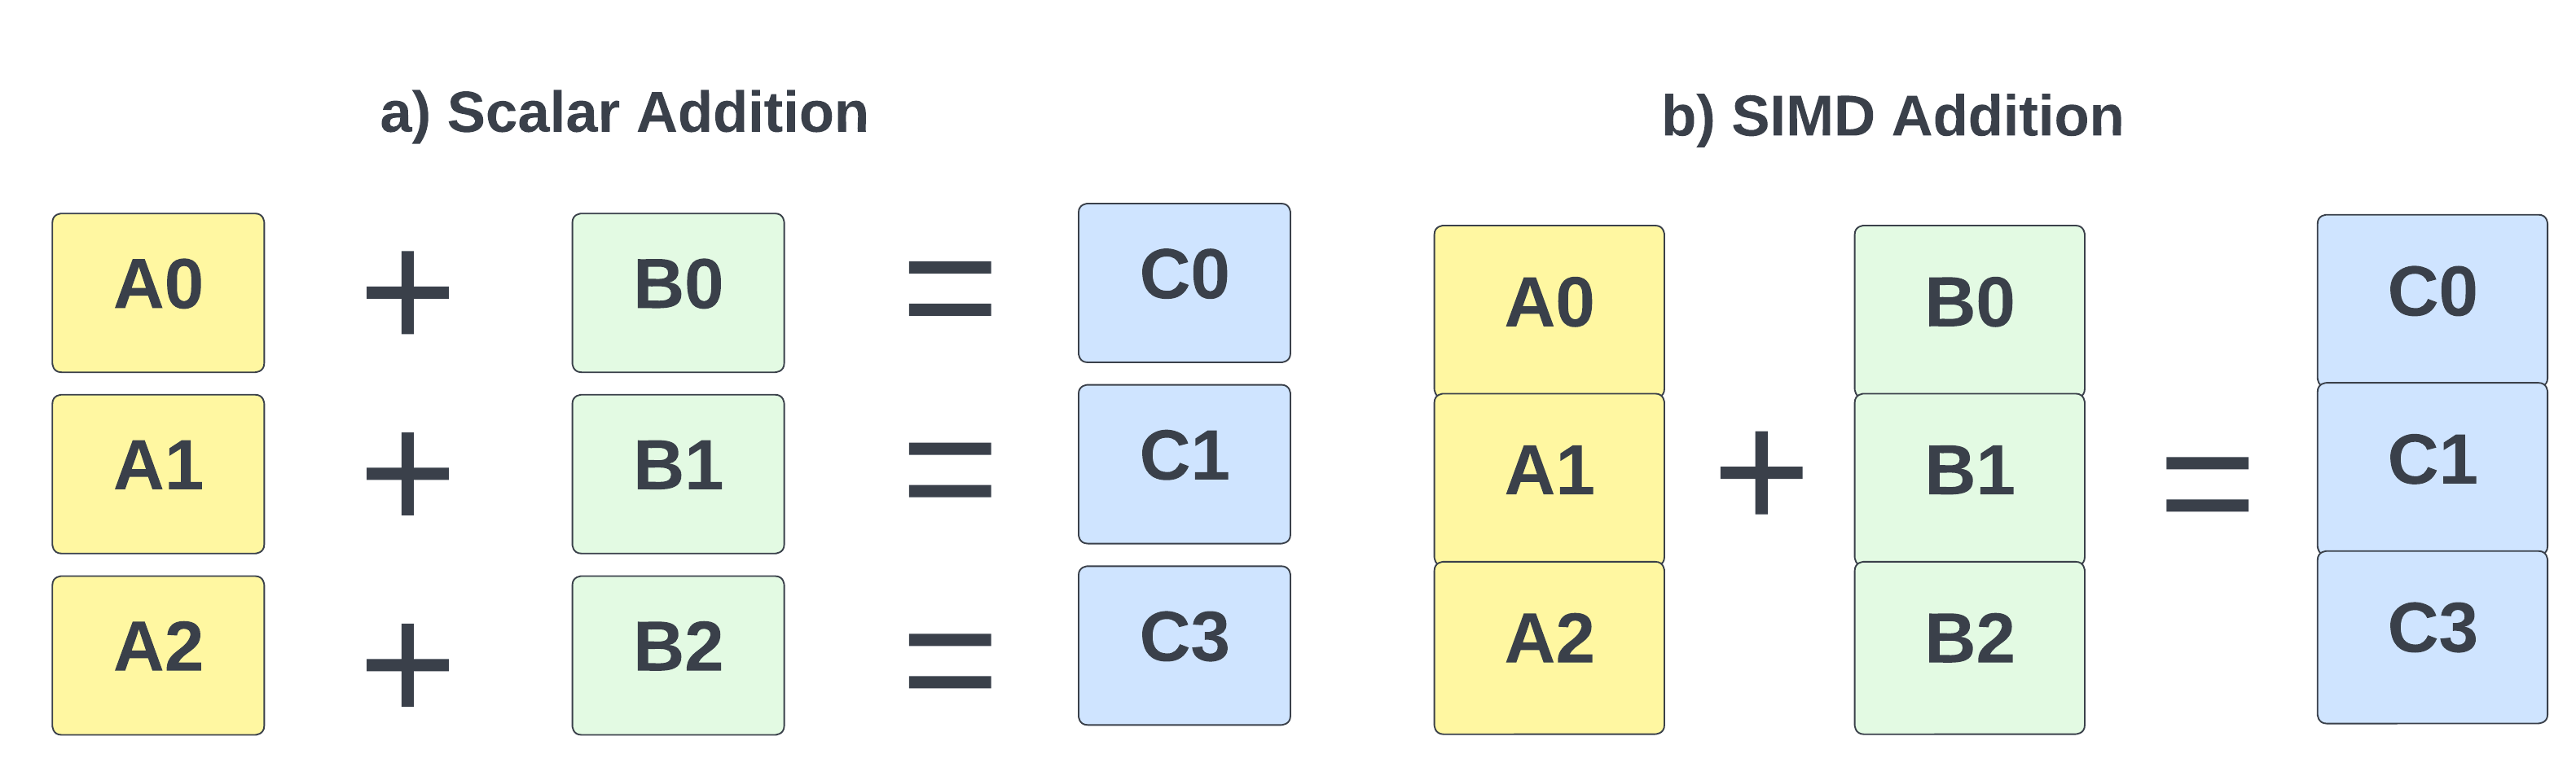
\includegraphics[width=\textwidth]{imgs/simd-add.png}
\caption[SIMD vs Scalar]{SIMD vs Scalar Operations \cite{simdscalar}}\label{fig:simdscalar}
\end{figure}

Figure \ref{fig:simdscalar} shows an example for addition using scalar and SIMD operations. Three scalar add instructions are executed sequentially to obtain the summation while only a single SIMD add instruction is required to achieve the same result.

